\documentclass[11pt, a4paper]{article}
\usepackage[T2A]{fontenc}
\usepackage[utf8]{inputenc}
\usepackage[english]{babel}

%% Sets page size and margins
\usepackage[a4paper,top=3cm,bottom=2cm,left=3cm,right=3cm,marginparwidth=1.75cm]{geometry}

%% Useful packages
\usepackage{amsmath, amssymb, amsthm,calc,mathabx}
\usepackage{systeme}
\usepackage{graphicx}
\usepackage[colorinlistoftodos]{todonotes}
\usepackage[colorlinks=true, allcolors=black]{hyperref}
\usepackage{wrapfig,lipsum,booktabs}
\usepackage{enumitem}
\usepackage{fmtcount}
\usepackage{multicol}
\usepackage{breqn}
\usepackage{setspace}
\usepackage{hyperref}
\usepackage {tikz}
	\usetikzlibrary {positioning}
	
\graphicspath{
	{Graphics/}
}

\newtheorem{theorem}{Theorem}
\newtheorem{definition}{Definition}
\newtheorem{lemma}{Lemma}
\newtheorem{prop}{Property}
\newtheorem*{remark}{Remark}

\setlength{\columnsep}{1cm}
\setlength{\parindent}{1em}
\setlength{\parskip}{1em}
\begin{document}
\begin{titlepage}
	\newcommand{\HRule}{\rule{\linewidth}{0.5mm}}
	\centering
	\textsc{\LARGE SRS 2019}\\[1cm]
	\HRule\\[1 cm]
	
	{\huge\bfseries Ransomware Research Project }\\[0.5 cm] 
	\HRule\\
    \vfill
			\Large
			\textit{Author:}
			 \textsc{Nikola Staykov}\\
             \vspace{2cm}
			\Large
			\textit{Supervisor:}
            \textsc{Yavor Papazov}
    \vfill	
	{\large\today}   
	\vfill
\end{titlepage}

\tableofcontents
\newpage
\begin{abstract}
		Malware is a type of computer virus, which encrypts the files on a given system and asks for a ransom in order for them to be decrypted. Ransomware authors have no way of knowing their victim's data value, or more precisely what people \textit{think} their data costs. They can, however, make small surveys before launching the main campaign, in order to estimate the aforementioned distribution. This paper explores a model in order to find the most suitable parameters for such a survey. This approach is key to finding the best price for the ransom.
\end{abstract}

\section{Introduction}
		Malware first appeared in 1989 in the form of the AIDS Troyan, aka PC Cyborg. It was not hard to decrypt after the files but this case set the ground for a lot of the modern threats. With the coming of the Internet age, ransomware returned with new power, 
\newpage
\section{Mathematical model}
	\subsection{Mathematical preliminaries}
		\begin{definition}[Normal distribution]
			Denoted with $N(\mu, \sigma)$, this is a type of continuous distribution, where:
			\begin{itemize}
				\item $\mu$ is the mean (in this case also mode and median)
				\item $\sigma$ is the standard deviation
				\item $\sigma^{2}$ is the variance
				
			\end{itemize}
			Its probability density function is
				$$\frac{1}{\sigma\sqrt{2\pi}}e^{-\frac{(x-\mu)^{2}}{2\sigma^{2}}}$$
		\end{definition}
	
			The graph of this function forms a curve, often called informally bell-curve. It has maximum $(x,f(x))$ at $(\mu, \frac{1}{\sigma\sqrt{2\pi}})$:
			\begin{center}
			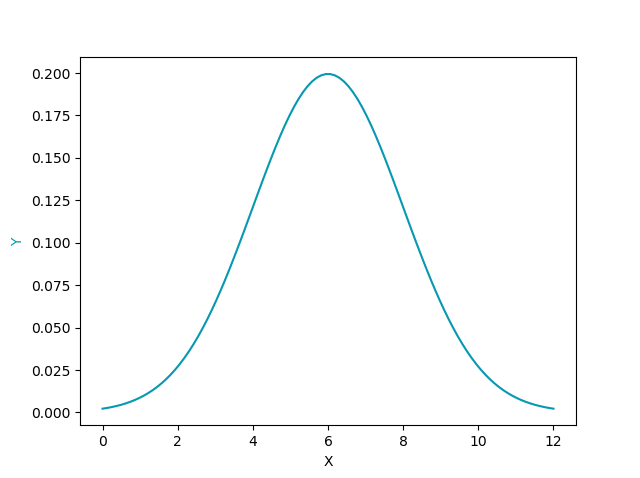
\includegraphics[width=0.5\textwidth]{Graphics/Normal_clean}
			\end{center}
		
		\begin{definition}[Standard value (aka Z-score)] Consider a normal distribution $N(\mu, \sigma)$. The standard value of a given $x$ is computed by $\dfrac{x-\mu}{\sigma}$ and evaluates how many standard deviations away from the mean the given value is.
			
		\end{definition}
	\subsection{The approach}
		This model describes the spread and calculates the optimal ransom for a ransomware attack, distributed exclusively via botnets, without the key component of spreading to every computer in the network. This variant of the attack is relatively cheap to initiate, but has low efficiency.\par
		We will treat the act of decrypting the data of a given computer as a service and the ransom, respectively, will be the price of the service. The parameters and distributions in this model will surely differ from standard market\par
		Consider the distribution for the willingness to pay (WTP) a given target group. By putting ourselves in the place of the malware authors, we can try to find out what the distribution is by examining samples of people and how they respond to a given price. This tests, however, cost us valuable time since the awareness of people rises constantly. So the question is, how many and how big test should we conduct in order to model the distribution with reasonable error and in the same time not lose too much time?
	\subsection{The model}
\section{Results}
\section{Further development}
\section*{Acknowledgments}
\nocite{*}
\bibliographystyle{unsrt}
\bibliography{Bibliography}
\end{document}